\section{Auswertung der Winkelabhängigen Messung}
Für die Winkelabhängige Koinzidenzmessung wurden die einzelnen Messpunkte analog zu den Kanälen des MCA im vorherigen Versuchsteil Normiert:
Nachdem die Fehler auf alle Messpunkte mittels der Formel \ref{zählfehler} bestimmt wurden, wurden diese mit den Messzeiten in Zählraten umgerechnet. Der Fehler auf die Zählrate wurde erneut mittels Formel \ref{fehlerfortp} Fortgepflanzt. Anschließend wurde der Messpunkt bei $-90^\circ$, welcher als Hintergrundmessung diente, von allen Messpunkten abgezogen.
Letztendlich wurde ein Kurvenanpassung einer Kurve der Form \ref{gaussian} angepasst, deren Parameter $\mu$ wieder der Mittelpunkt von dieser ist. Es wurden nur die Fehler der Zählrate berücksichtigt, denn selbst der kleinste Fehler hier ist deutlich größer als die kleinsten Winkelfehler. Nach Abbildung \ref{Winkelbild} liegt der Mittelpunkt des Fits bei $-0.8\pm0.11$ Grad, wobei er für $0^\circ$ erwartet wurde. 

\begin{figure}[h]
	\centering
	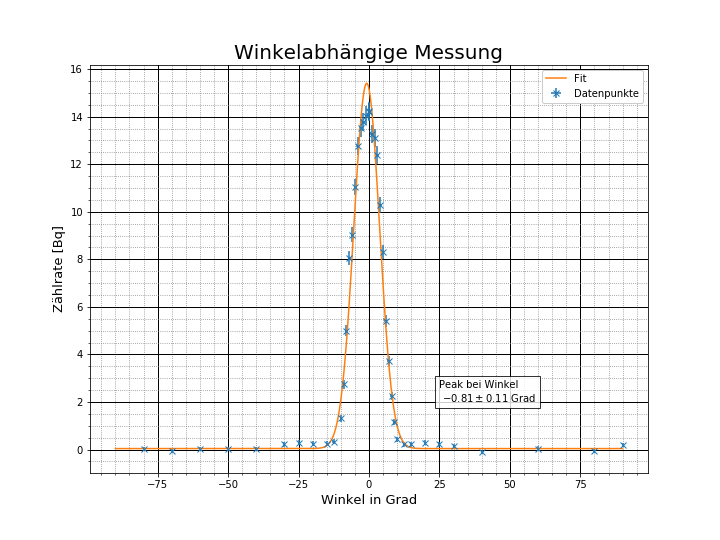
\includegraphics[scale=0.7]{Bilder/Winkel}
	\caption[Winkelmessung]{\small Die Zählraten gegen den Winkel, an welchem sie gemessen wurden aufgetragen. Der Fit zum Peak ist auch eingezeichnet sowie die Position der Spitze des Peaks.}
	\label{Winkelbild}
\end{figure}
